
\documentclass[10pt, a4paper, twoside]{article}
\usepackage[utf8]{inputenc}
\usepackage{authblk}
\usepackage{multicol}
\usepackage{abstract}
\usepackage{xcolor}
\usepackage[a4paper, total={6in, 8in}]{geometry}
\usepackage{graphicx}
\usepackage{newfloat}
\usepackage{hyperref}
\usepackage{csvsimple}
\usepackage{lscape}
\usepackage{makecell}
\usepackage{fancyhdr}

\DeclareFloatingEnvironment[name={Supplementary Figure},fileext=lsf,listname={List of Supplementary Figures}]{suppfigure}

\setlength{\columnsep}{1cm}

\pagestyle{fancy}

\graphicspath{{../Figures/}}
\title{Impact of cross-border-associated cases on the SARS-CoV-2 epidemic in Switzerland from June to September 2020}
\renewcommand*{\Authfont}{\small}
\author[1]{Martina L. Reichmuth}
\author[1,2]{Emma B. Hodcroft}
\author[1,3]{Julien Riou}
\author[2,4]{Richard A. Neher}
\author[5,6]{Niel Hens}
\author[1*]{Christian L. Althaus}

\renewcommand*{\Affilfont}{\scriptsize}
\affil[1]{Institute of Social and Preventive Medicine, University of Bern, Bern, Switzerland}
\affil[2]{Swiss Institute of Bioinformatics, Basel, Switzerland}
\affil[3]{Federal Office of Public Health, Liebefeld, Switzerland}
\affil[4]{Biozentrum, University of Basel, Basel, Switzerland}
\affil[5]{Interuniversity Institute for Biostatistics and statistical Bioinformatics, Data Science Institute, Hasselt University, Hasselt, Belgium}
\affil[6]{Centre for Health Economics Research and Modelling Infectious Diseases, Vaccine and Infectious Disease Institute, University of Antwerp, Antwerp, Belgium}
\affil[*]{Correspondence: christian.althaus@ispm.unibe.ch}


\renewcommand{\abstractnamefont}{\small}
\renewcommand{\abstracttextfont}{\footnotesize} 


\date{}
\pagenumbering{arabic}
\begin{document}
\maketitle

\begin{abstract}
\noindent 
\textbf{Introduction:} In Switzerland, the severe acute respiratory syndrome coronavirus 2 (SARS-CoV-2) epidemic grew from a few dozen confirmed cases to several hundred cases per day during summer 2020. 
During this time Switzerland holiday travel was largely allowed without quarantine. 
So far, the impact of potential cross-border-associated cases (imports) on the national epidemic dynamics remains unclear. 
Our objective was to assess the impact of imports on the epidemic.\\
\textbf{Method:} For the purpose of this study, we used individual data on positive cases reported to the Swiss Federal Office of Public Health from 1 June to 30 September 2020. 
Data included age, sex, date of diagnosis or registration, if hospitalised or deceased, date of hospitalisation, date of death, and the most likely country of exposure.
We fitted a negative binomial generalised linear model to the daily number of confirmed cases, hospitalisations, and deaths reported to the Swiss FOPH to estimate the epidemic growth rate. 
We then used a stochastic branching process model that accounts for superspreading in transmission of SARS-CoV-2 to simulate epidemic trajectories using different values for the effective reproduction number $\mathcal{R}_e$ (0.8-1.2) and number of imports (3,304-15,154).\\
\textbf{Results:} From June to September 2020, 23,199 SARS-CoV-2 cases were reported. 
For 12,259 cases (53\%) the most likely country of exposure was reported. 
Of these, 3,304 (27\%) declared that exposure was most likely outside of Switzerland.
In absence of imports, we estimated an epidemic growth rate of 0.023 (95\% confidence interval: 0.021-0.024) per day corresponding to a $\mathcal{R}_e$ of 1.124 (95\%-CI: 1.12-1.13).
We found a larger number of imports over period would correspond to lower values of $\mathcal{R}_e$ to fit the observed dynamic. 
For example, 3,304 imports (as reported) would have been sufficient to account for the observed epidemic dynamics despite $\mathcal{R}_e < 1$, i.e., a value below the critical threshold.\\
\textbf{Discussion:} In Switzerland, imports had a considerable impact on the national dynamics and can explain the sustaining of the SARS-CoV-2 epidemic during summer 2020. 
Our results underline the importance of improved surveillance for international travellers in order to better control the spread of SARS-CoV-2.\\ 

\clearpage
\end{abstract}
\normalsize


\begin{multicols}{2}
\section{Introduction}

\rhead{Confidential, please delete!}
\lhead{ }
The dynamics of infectious diseases depend on the pathogens, their host, and environmental factors such as humidity and temperature.\cite{leung_transmissibility_2020} 
At the beginning of 2020 the severe acute respiratory syndrome coronavirus 2 (SARS-CoV-2) was introduced to many countries around the world, which shortly afterwards led to the SARS-CoV-2 pandemic.
Since then many have been aiming to minimise the SARS-CoV-2 cases and associated deaths.

In Switzerland the first case was reported on $25^{th}$ February 2020.% https://www.bag.admin.ch/bag/en/home/das-bag/aktuell/medienmitteilungen.msg-id-78233.html
Until $31^{st}$ May 2020, 30,883 COVID-19 cases were reported to the Swiss Federal Office of Public Health (SFOPH). %  https://www.bag.admin.ch/bag/de/home/krankheiten/ausbrueche-epidemien-pandemien/aktuelle-ausbrueche-epidemien/novel-cov/situation-schweiz-und-international.html
During the summer of the northern hemisphere, warm weather was beneficial to contain the number of SARS-CoV-2 cases.\cite{neher_potential_2020} 
Nevertheless, the SFOPH reported an increase of the SARS-CoV-2 epidemic from a few dozen confirmed cases per day in early June 2020 to several hundred cases per day by the end of September 2020.
After an unprecedented closures - closure of public institutions, leisure facilities, schools and universities, mandatory home office and closing of borders -  in April and May 2020, Switzerland and other European countries had reopened their borders to allow for travel. 
In Switzerland borders were reopened on the $15^{th}$ of June 2020 to EU Schengen states. 
To note, Switzerland is a rather small country with 8,5 millions citizens in the heart of Europe - with boarders to Germany, France, Italy, Austria, and Principality of Liechtenstein.
Many different countries might easily be visited by the Swiss and vice-versa many citizens from other countries might visit Switzerland. 

In spring 2020, imports were most likely responsible for the pandemic and a high proportion of cases in many countries.\cite{russell_effect_2021}
With a high number of introductions it was likely that the local effective reproduction number $\mathcal{R}_e$ with which the dynamic can be quantified was overestimated at that time.\cite{roberts_early_2011}
The $\mathcal{R}_e$ is the average number of secondary cases per infectious case in a population with a given state of susceptibility, with particular measures of prevention and control in place. 
When $\mathcal{R}_e > 1$ the incidence of infections will increase, when $\mathcal{R}_e = 1$ it will remain stable, and when $\mathcal{R}_e < 1$ it will decrease. 
The $\mathcal{R}_e$ estimated from the local dynamics can be interpreted as a measure of the average intensity of local transmission if preventive and control measures are in place that aim to limit potentially infectious contacts, i.e. imports should not be influence the $\mathcal{R}_e$ estimated.
However, the number of reported cases in a given area does not only depend on local transmission, but also on imports.
If a large proportion of reported cases were exposed abroad, the resulting estimate of $\mathcal{R}_e$ will be overestimated as local transmission is lower due to effective control measures.
In the absence of travel restrictions, countries can expect cross-border-associated cases.\cite{russell_effect_2021} 
A phylogenetic analysis could prove the assessment of cross-border-associated cases.\cite{hodcroft_emergence_2020}
In summer 2020, the SARS-CoV-2 variant, 20A.EU1, that most likely originated in Spain spread multiple times to several other countries including Switzerland.\cite{hodcroft_emergence_2020}
This revealed failures in travel control during a pandemic, e.g. there have been trips to higher incidence country without adequate contact tracing.\cite{hodcroft_emergence_2020}


We aimed to evaluate the effect of cross-border-associated cases on the local SARS-CoV-2 incidence and epidemic growth in Switzerland between June and September 2020. 
Therefore we analysed reported SARS-CoV-2 cases and the most likely country of their exposure, i.e., where they had been the last 14 days before they got tested or began to have symptoms. 
We compared this data to different epidemic scenarios using a stochastic branching model to finally quantify the effect of cross-border-associated cases in Switzerland during summer 2020.


\section{Method}

\subsection{Data}
We analysed surveillance data of the SARS-CoV-2 epidemic in Switzerland from $1^{st}$ June to $30^{st}$ September 2020. 
For the purpose of this study, we used individual data on positive cases reported to the Swiss FOPH. 
Data included for each case: age, sex, date of diagnosis or registration, if hospitalised or deceased, date of hospitalisation, date of death, and the most likely country of exposure, i.e., a country where they had been the last 14 days before they got tested or began to have symptoms.
We considered the 23 most frequently reported countries of exposure (including Switzerland).
Other countries (mentioned less than ten times) were grouped to 'others'.
We have grouped individuals into three categories based on their age: $<$21 years, 21-64 years and older adults $>$64 years.


\subsection{Inferring growth rates and $\mathcal{R}_e$}
\label{marker}

We fitted three separate negative binomial generalised linear models to the daily number of
\\1) reported cases of SARS-CoV-2 infection,
\\2) COVID-19-related hospitalisations and
\\3) COVID-19-related deaths\\
starting on $1^{st}$ June to $30^{th}$ September 2020. 
The models were adjusted for the lower counts observed during weekends.
These growth rates were combined into a unique epidemic growth rate $r$ using
\[ \frac{ \sum_{i=1}^n ( \frac{ r_i}{\sigma_i^{2}} )}{  \sum_{i=1}^n \frac{1}{\sigma_i^{2}}}, \]
and the standard error of the weighted r was calculated as
\[ \sqrt{\frac{ 1 }{\sum_{i=1}^n \sigma_i^{-2}}}\]%https://en.wikipedia.org/w/index.php?title=Weighted_arithmetic_mean&action=edit&section=6
and resulted in one weighted estimate of the average daily growth rate over the whole period.
This approach assumes a constant growth rate and ignores potential acquired immunity.

Growth rate, $r$, and reproduction number can be mutually calculated taking into account the generation time, i.e. time between the infection of a primary case and one of its secondary cases.\cite{svensson_note_2007}
To calculate $\mathcal{R}_e$ from $r$, we used a calculation that estimates $\mathcal{R}_0$ as potential acquired immunity was minimal during the time of interest in Switzerland.
If the generation time follows a gamma distribution with shape $\alpha$ and rate $\beta$, the value of $\mathcal{R}_0$ (here also $\mathcal{R}_e$) is given by \[ (1 + \frac{r}{\beta} )^\alpha.\cite{wallinga_how_2007,krauer_heterogeneity_2016} \]
For SARS-CoV-2, the generation time was estimated to have a mean $\mu= 5.2$ days and a standard deviation $\sigma = 1.72$.\cite{ganyani_estimating_2020}
Parameters $\alpha$ and $\beta$ were estimated from $\mu$ and $\sigma$ as $\frac{\mu^2}{\sigma^2 }$ and $\frac{\mu}{\sigma^2}$, respectively.\textcolor{red}{[citation?]}

\subsection{Epidemic simulation}

We simulated epidemics for the period of interest, $1^{st}$ June to $30^{th}$ September 2020, using a stochastic branching process model that also accounts for individual variation in transmission of SARS-CoV-2.
Within this framework, the distribution of secondary cases was described with a negative binomial distribution with mean $\mathcal{R}_e$ and variance $\frac{\mathcal{R}_e}{1+\frac{\mathcal{R}_e}{k}}$ where $k$ is the over-dispersion parameter. 
We considered different $k$ values within a range of 0.49 to 0.52.\cite{laxminarayan_epidemiology_2020}
More precisely, considered $10^3$ values of $k$ were normal distributed with a mean of 0.51 (Table \ref{t1}).
The simulations were initiated using cases calculated from the fitted negative binomial model to the daily counts of 1) reported cases of SARS-CoV-2 infection.
More precisely, seeds for each simulation were randomly chosen from a range of minimum and maximum number of potential cases per day. 
This range of potential cases per day was derived from estimates for May $25^{th}$ to $31^{st}$ using the negative binomial model of 1) reported cases of SARS-CoV-2 infection. 
These estimates were expanded to include their 95\% confidence interval (CI). 
Finally, a random number of cases was chosen for each day from May $25^{th}$ to $31^{st}$ and for each simulation (sampling with replacement). 

Onwards local transmission was simulated using $\mathcal{R}_e$ values ranging from 0.8 to 1.2 (Table \ref{t1}).
Within this range we considered $10^3$ uniformly distributed values.
Imports were added on the day that they were reported to the FOPH to the pool of local infectious cases throughout the simulation, and thus initiating new branches of local transmission.
Due to missing data, extrapolated number of imports was estimated.
We multiplied the number of imports by $1+ \frac{\Sigma ~of ~cases ~with ~known ~origin }{\Sigma ~of ~all ~confirmed ~cases}$.
In total, we considered seven scenarios of number of imports that resulted from multiplying by zero, one, two, three, weighted imports, and combinations (Table \ref{t1}).

All simulations could not exceed $10^6$ cases during the time of interest.
For each scenario, we computed the 95\% CI of cumulative cases, final size, and the effective growth rate.

\begin{table*}[h]
	\centering
\caption{Summary of parameter values used for simulating epidemics.*Normal distribution with a mean of 0.51. **Reported imports were weighted with $1+ \frac{\Sigma ~of ~cases ~with ~known ~origin }{\Sigma ~of ~all ~confirmed ~cases}$ or multiplied with 0, 1, 2 or 3.}
\label{t1}
\begin{tabular}{clll}
	\hline
	Parameter & Description & Values considered & Sampling strategy\\
	\hline
	$\mathcal{R}_e$ & Effective reproduction number & 0.8 - 1.2 & $10^3$ uniformly distributed\\
	$k$ & Over-dispersion parameter & 0.49 - 0.52 & $10^3$ normally distributed*\\
	$n$ & Seeds & 12 - 32 per day & for previous 7 days\\
	$I$ & Imports & 0 - 15,154 & seven scenarios**\\
	$Z$ & Limitation & $10^6$ & Maximum of cumulative cases\\
	\hline
\end{tabular}
\end{table*}

\subsection{Statistics}
We validated our simulations using the final size, cumulative cases, and the growth rate.
For all variables we used a 95\% credible interval (CI) and validated it regarding the 95\% CI of the reported values and their 95\% CI. \textcolor{red}{need help here}.
The 95\% CI for reported final size was calculated using $10^4$ simulations of the final size using as seed the second last day of reported cases.
The 95\% CI for reported cumulative cases was calculated using normal distribution $10^4$ simulations, mean of reported cumulative cases, and standard deviation of 
%\[ \sqrt{\frac{ 1 }{\sum_{i=1}^n \sigma_i^{-2}}}\]
\[ \frac{\mathcal{R}_e}{\frac{1+ \mathcal{R}_e} {k}},\]
where for $k$ and $\mathcal{R}_e$ the mean was used.
The 95\% CI for inferred growth rate and $\mathcal{R}_e$ was described in more detail in section \nameref{marker}.
We used two-sided t-test to assess the age differences in relation to the different most likely countries of exposure.
As a sensitivity analysis left and- right sided t-test were performed.
The incidence of reported cases was calculated for each day, including one week, i.e. mean of three days before and after the date of interest.
The estimated mean of incidence was divided by 8,697,905 (number of Swiss citizens see \href{https://www.worldometers.info/world-population/switzerland-population/}{here}) and multiplied by 100,000.

All analyses were preformed using $R ~v.4.0$ and package \texttt{MASS, MCMCglmm, doParallel, foreach, lubridate, reshape2, ggplot2, ggpubr, grid, gridExtra, wesanderson } \textcolor{red}{cite!}.\cite{r_core_team_r_2020,venables_modern_2002}

\section{Results}
In total 23,199 cases were reported to the Swiss FOPH between $1^{st}$ June to $30^{th}$ September, 2020. 
Of them, 13,929 (48\%) were female and 14,985 (52\%) were male.
For nine individual their gender was not known.
For 12,259 (53\%) cases the most likely country of exposure was reported.
Of them, 3,304 (27\%) reported an exposure abroad (Table \ref{t2}); Figure \ref{f1}).
Of all exposures that were likely to happened abroad, 1,562 (56\%) were female and 2,000 (56\%) were male.
The peak of reported imports was on $6^{th}$ of September 2020 (Figure \ref{f1}c,d).

\begin{figure*}[h]
\centering
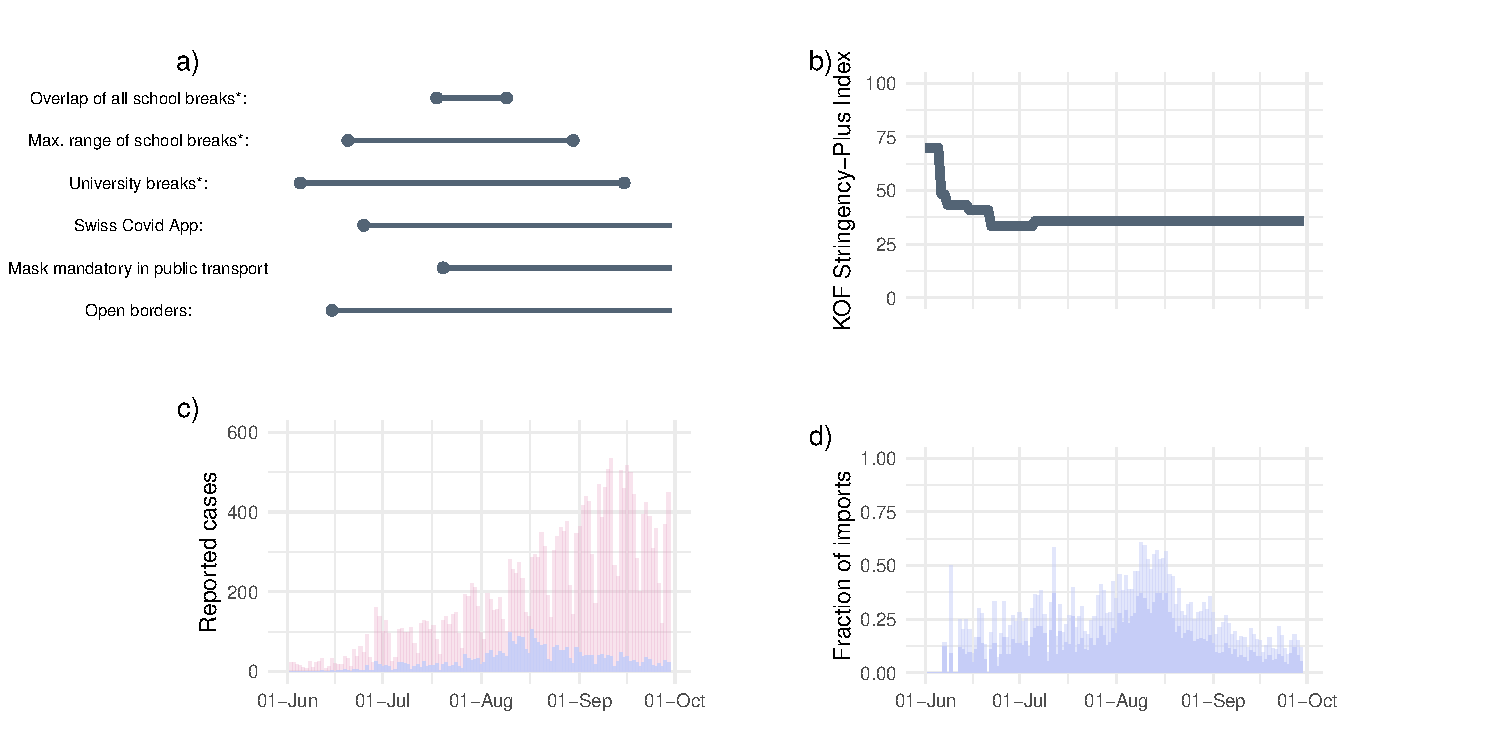
\includegraphics[scale=0.5]{Figure1_2021-04-19.pdf}
\caption{Reported cases and major events in Switzerland: a) Bars visualise major events from $1^{st}$ June to $30^{th}$ of September. b) Line visualises the KOF stringency plus index that records the stringency of COVID-19 policy measures in Switzerland over time. The values range from 0 (= no measures) to 100 (= full lockdown) (see \href{https://kof.ethz.ch/en/forecasts-and-indicators/indicators/kof-stringency-index.html}{here}. c) Blue bars show cross-border-associated cases per day and pink bars show all reported cases. d) Transparent and light blue bars show the fraction $\frac{\Sigma ~of ~cases ~with ~origin~aboard }{\Sigma ~of ~cases ~with ~known ~origin }$  and the dark blue bars show the fraction $\frac{\Sigma ~of ~cases ~with ~known ~origin }{\Sigma ~of ~all ~confirmed ~cases}$. $*$Official breaks of universities and schools might vary for different subjects and between different schools and cantons, respectively. More details on quarantine measures in Table \ref{t2} and \href{https://www.fedlex.admin.ch/eli/cc/2021/61/de}{here}.}
\label{f1}
\end{figure*}

The study population was 34 (interquartile range (IQR): 24-50, range: 0-104) years (Table \ref{t2}).
Individuals that had an exposure abroad were 31 (IQR: 23-48; range: 0-88) years.
Individuals who stated that Switzerland was the only country of exposure were 35 (IQR: 24-51; range: 0-102) years.
Individuals that did not report their most likely country of exposure were 35 (IQR: 25-51; range: 0-104) years.

Different age categories were more likely to visit some countries during summer (Table \ref{t2}); Supplementary Figure \ref{sf3}).
The age of individuals that reported that their most likely country of exposure was in France, Croatia, Kosovo, Italy, Serbia, Spain, Malta, Greece, North Macedonia, Bosnia and Herzegovina, Hungary, Czech Republic, Slovenia  or did not report the most likely country of exposure, was significantly different compared to cases who had only an exposure in Switzerland (Table \ref{t2}; Supplementary Figure \ref{sf3}):
More precisely, individuals were significantly older (p-value $<0.05$) if they reported to also have been in Kosovo, Serbia, North Macedonia or Bosnia and Herzegovina and not only in Switzerland.
Contrary, individuals were significantly younger (p-value $<0.05$) if they reported to also have been in France, Croatia, Italy, Spain, Malta, Greece, Hungary, Czech Republic, or Slovenia and not only in Switzerland.

Beginning of June 2020, Switzerland had an incidence of 0.17 per 100,000 citizens and at the end of September 5.36.
The latter was also the maximum value during the time of interest.
Assuming no imports, we estimated an epidemic growth rate of 0.027 (95\%-confidence interval (CI): 0.025-0.029) per day and a $\mathcal{R}_e$ of 1.149 (95\%-CI: 1.138-1.16) for June to September.
The weighted growth rate was 0.023 (95\%-CI 0.021-0.024) per day and $\mathcal{R}_e$ 1.124 (95\%-CI: 1.116-1.133) for the time of interest. % Reff is narrow, I used the growth rate 95%CI with following calculation:  $(1 + \frac{r}{\beta} )^\alpha$. 
\textcolor{blue}{With the branching process we estimated a $\mathcal{R}_e$ of 1.129 (95\%-CI: 1.087-1.171).
Accounting for imports requires to re-evaluate the intensity of local transmission (i.e. the value of $\mathcal{R}_e$) to match the observed dynamics of SARS-CoV-2 in summer 2020.
We assume that imports were equally likely to transmit as local cases.
With 3,304, 5050, 6608, 9912,10096, or 15154 imports a $\mathcal{R}_e$ of 0,974 (95\%-CI: 0.932-1.009),  0.921 (95\%-CI: 0.880-0.960), 0.881 (0.881-0.924), 0.860 (0.826-0.881), and 0.812 (0.801-0.828), respectively explains the local epidemic (Table \ref{t2}; Supplementary Figure \ref{sf1}).}

\begin{figure*}[h!]
\centering
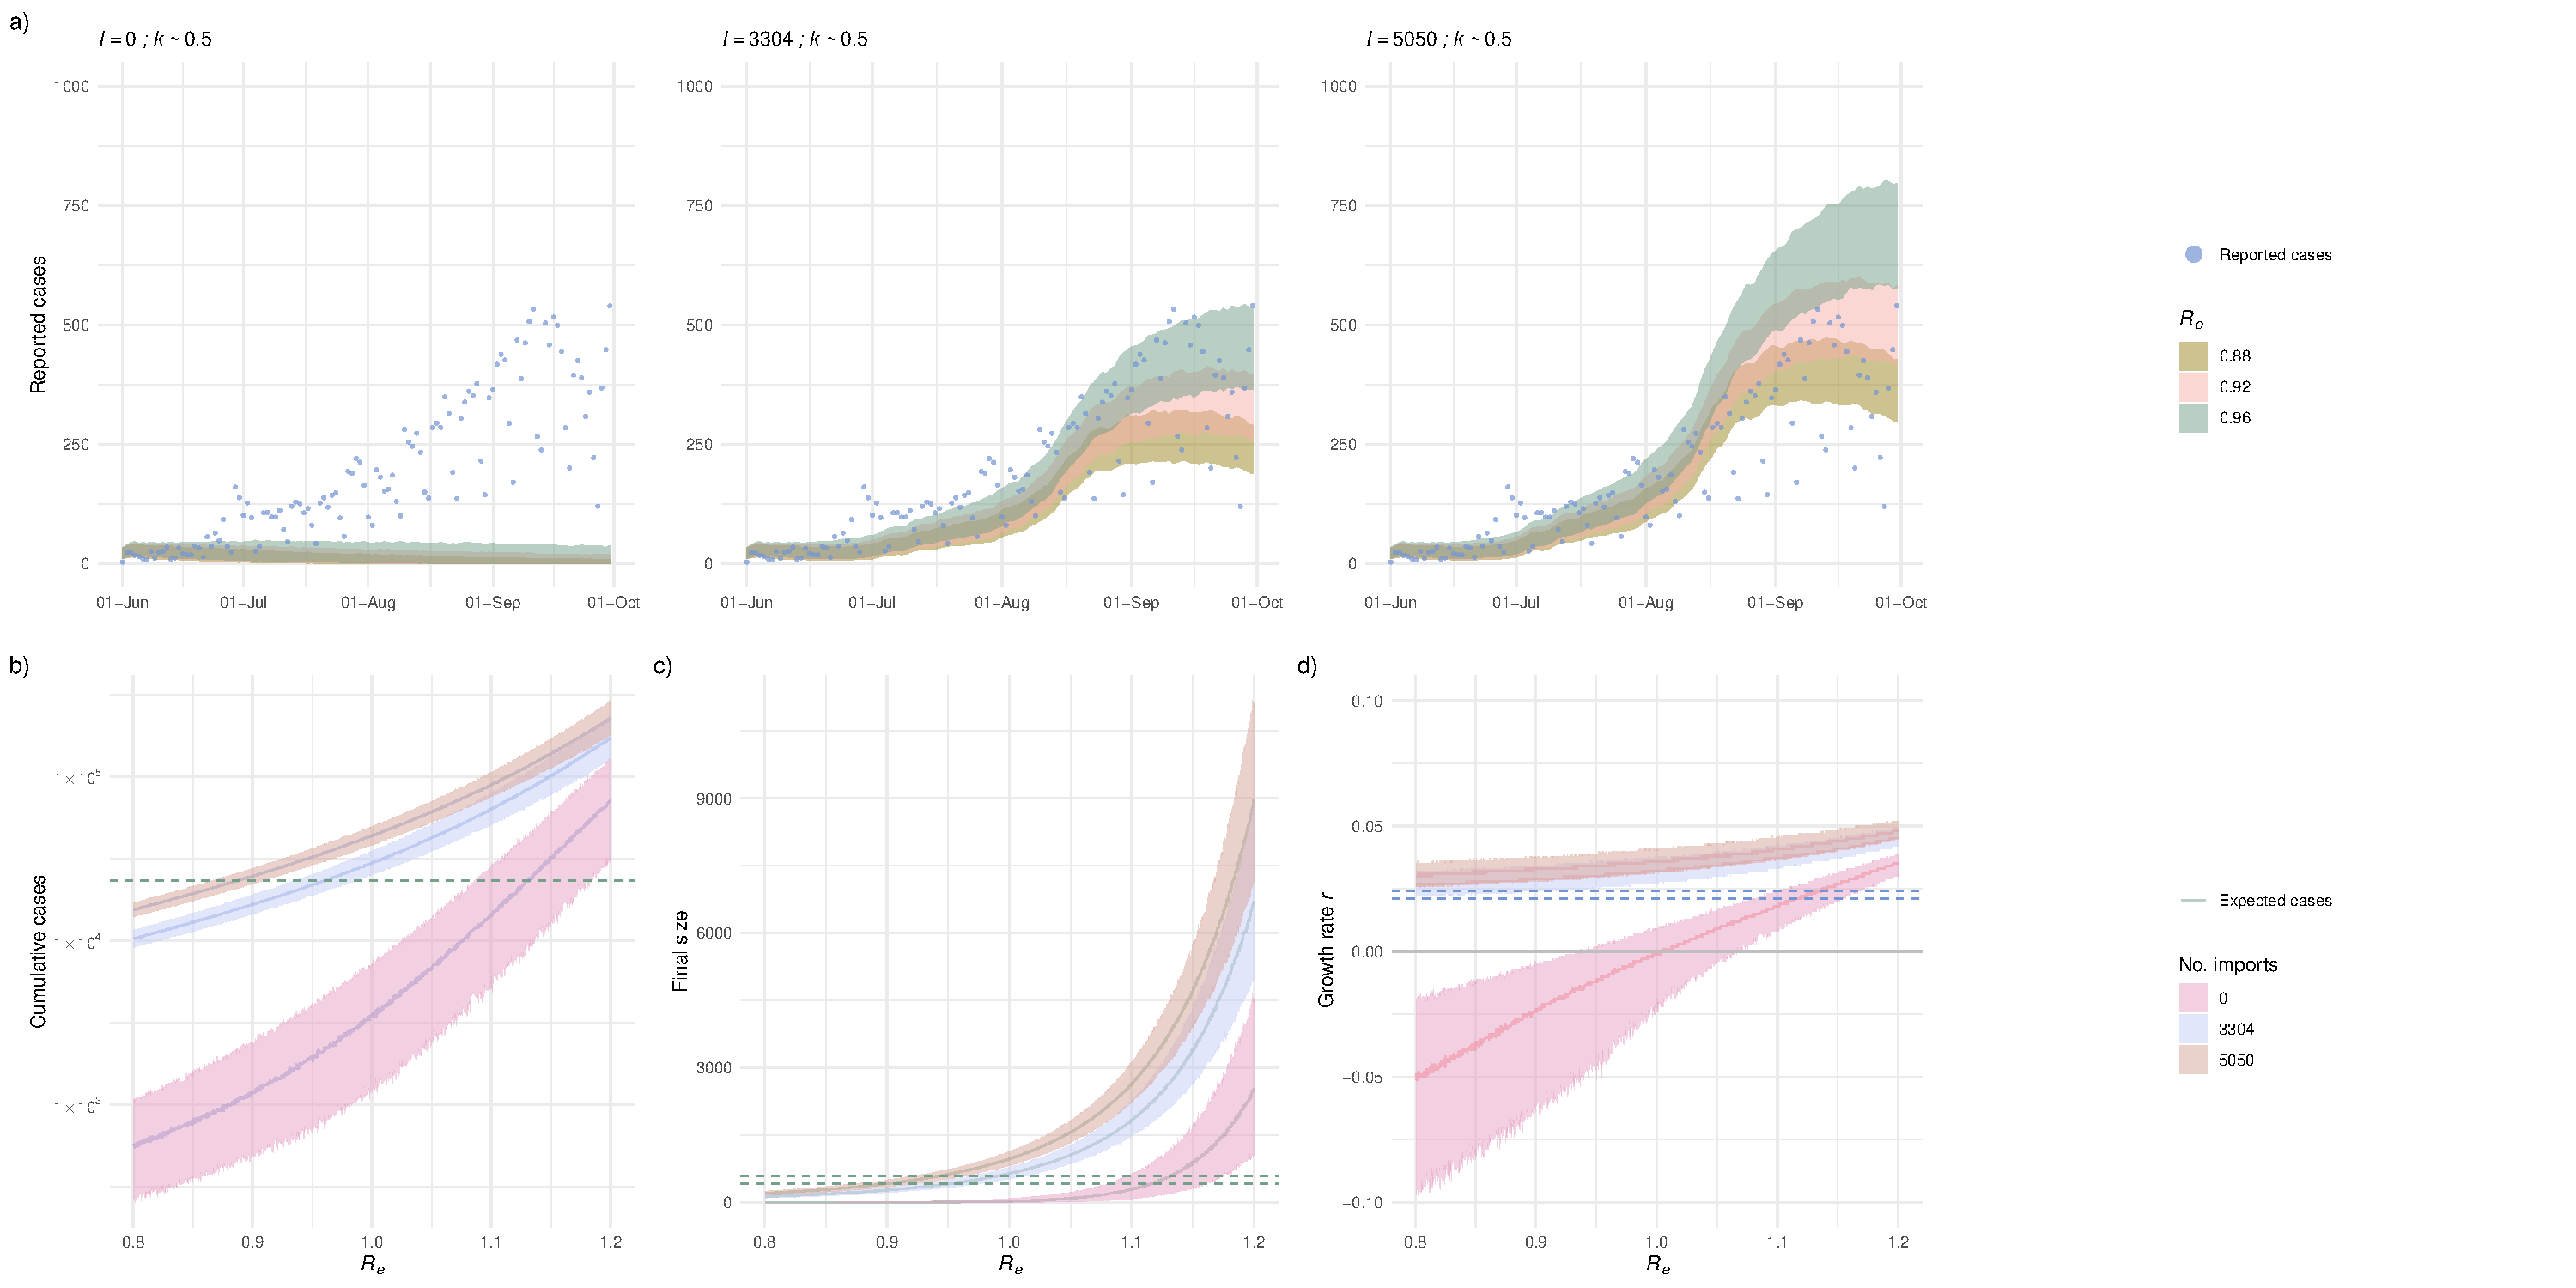
\includegraphics[scale=0.3]{Figure2_2021-04-19.pdf}
\caption{Impact of imports on the epidemic.
a) Green dots are reported cases per day and the curves represent 95\%-CI of simulated cases per day.
b) Cumulative cases with zero, 3304, and 5,050 imports, dashed line represent reported cases during $1^{st}$ of June to $30^{th}$ of September 2020 (dashed line represent the 95\%-CI). 
c) Final number of cases with zero, 3304, and 5,050 imports, dashed line represent the 95\%-CI of reported cases on $30^{th}$ of September 2020.
d) y-axis the epidemic growth rate; x-axis $\mathcal{R}_e$ values; intervals represents 95\%-CI.
Abbreviations: I, number of imports; CI, confidence interval}
\label{f2}
\end{figure*}
\end{multicols}
\begin{landscape}
\global\pdfpageattr\expandafter{\the\pdfpageattr/Rotate 90}
\input{{../data/table2.tex}}
\end{landscape}
\begin{multicols}{2}
\global\pdfpageattr\expandafter{\the\pdfpageattr/Rotate 0}

\section{Discussion}
The SARS-CoV-2 epidemic in Switzerland grew from a few dozen confirmed cases per day in early June 2020 to several hundred by the end of September 2020. 
Ignoring cross-border-associated cases the $\mathcal{R}_e$ was above one for the time of interest. 
In summer 2020, however, around a quarter of cases that have been reported to the Swiss FOPH were cross-border-associated cases.
We also found that different age groups were exposed to the SARS-CoV-2 in different countries abroad.
Further, with our stochastic simulations we showed that the local epidemic had a $\mathcal{R}_e$ below one, i.e. a value below the critical threshold.
At the end of summer 2020, the reported cases stabilised (also in the simulations if $\mathcal{R}_e <1$).
Thus, cross-border-associated cases and their local spread was one of the leading forces that led to several hundred cases per day within three months, i.e., by the end of September 2020. 
Consequently, the effect of cross-border-associated cases cannot be ignored in understanding and regulating a local epidemic (during a pandemic).

Our method has limitations that need to be addressed.
In our stochastic model, we did not account for a saisonal effect of the SARS-CoV-2, different restrictions carried out, social contact pattern or age-related mixing patterns.
We were not interested to simulated single transmission chains.
Our model was calibrated to assess the impact of cross-border-associated cases on an epidemiological, i.e. population-based, level.
We did not consider the geographical region of residence, i.e. the canton, we found no evidence of relevant different rates of cross-border-associated cases (Supplementary Figure \ref{sf4}).
Our approach assumes a constant growth rate over the summer period and ignores immunity, which we consider acceptable during this low prevalence and incidence period.
The SFOPH reported 30,883 cases before $1^{st}$ June and 23,199 more until $30^{th}$ September.
Growth rates, can be calculated for different intervals, e.g., one week or months, we decided assumes a constant growth rate.
This was more appropriate to calculate the overall influence of cross-border-associated cases.
The stochastic branching process was calibrated to simulate the number of reported cases.
Stochastic effects have been showed to play an important role in determining the outcome of the outbreak.\cite{althaus_ebola_2015}

Further, it is unlikely that all SARS-CoV-2cases have been tested, but in Switzerland all cases tested have been reported to the FOPH.
Studies reported about a two-fold (or more) underreporting of SARS-CoV-2 infections.\cite{Li_substantial_2020,Wu_substantial_2020}
The degree of under-ascertainment can not be evaluated for the used surveillance data.\textcolor{red}{[true?]}
Moreover, there is a delay of infection to testing and reporting.
We ignored this delay for all cases.
Thus, our results reflect the day of testing and reporting and not the start of infection.
During the time of the study, testing was free and mandatory for symptomatic cases, but not for asymptomatic cases.
However, if they had contact with a positive person they were required to do isolate and test themselves. 
The contact tracing was provided either by the person themselves, through authorities or the Swiss Covid app (launched on $15^{th}$ June 2020).\cite{salath_early_2020}
As our study period covered only summer it is be expected that seasonality played a role.
However, people were more active in summer than in winter and likely more optimistic about the pandemic (at the end of summer), which likely resulted in more social contacts than before.

With our stochastic branching model, we were able to confidentially simulate the Swiss epidemic.
Also in other countries, travel had a strong impact on the local epidemic.\cite{russell_effect_2021,hodcroft_emergence_2020}
Linka et al., showed a correlation between air travel, driving, walking, and transit mobility and the $\mathcal{R}_e$.\cite{linka_reproduction_2020}
Unfortunately, social contact pattern or age-related mixing patterns are missing for this time in Switzerland.
Such information of a representative study population, like established by the Co-Mix study, are needed to better understand the social dynamics.\cite{coletti_comix_2020}
However, close contact alone is not responsible for SARS-CoV-2 transmission.
Some transmission cluster were linked to indoor crowded spaces which underlines the possibility of aerosol (and droplet) transmission.\cite{tang_aerosol_2020}
Nevertheless, tracking contact patterns, i.e., behaviour, can give a more rapid assessment of the impact of physical distancing measures than routine epidemiological surveillance.\cite{jarvis_quantifying_2020}
This highlights the importance of implementing and following up the Co-Mix study and other studies.
Our study indicated that to understand the spread of SARS-CoV-2  age-related mixing patterns need to be known.
Our study design was appropriate for our research question.
Nevertheless, there is a need of analysis that include several more variables, such as age-contact pattern, saisonal- or climate changes.
These will help to more precisely forecast future outbreaks and pandemics.

Our results are important to derive travel strategies, including mandatory quarantine and test strategies for the coming summer 2021.
It is likely that (global) herd immunity will not be achieved in the summer, so existing measures such as testing and physical distancing remain important to keep cases low.
In addition, there is still uncertainty about asymptomatic cases.\cite{nogrady_what_2020}
Studies found the proportion of asymptomatic cases to be 17\% (or 20\%) and 1/4 less transmissible.\cite{byambasuren_estimating_2020,buitrago-garcia_occurrence_2020,bi_household_2020}
It should be an option to test all people that cross borders and give them the option of reduced quarantine for negative cases.\cite{ashcroft_quantifying_2021}
In the summer of 2020, only five countries from 21 countries with at least a dozen cross-border-related cases were on the mandatory quarantine list at the beginning of July.
A handful of countries of these 21 had not been on the list during summer.
Mandatory quarantine and testing might reduce the willingness to travel as the effort and awareness of the SARS-CoV-2 pandemic remains.
Thus, travel mobility can be reduced, and cross-border-associated cases and their local spreading are minimised through testing and mandatory quarantine.
%https://www.eurosurveillance.org/content/10.2807/1560-7917.ES.2020.25.4.2000057/?crawler=true. 

Switzerland is a relatively small country with a few million citizens, but due to its location (and its wealth) there is a high potential for travel to have a huge impact on the epidemic.
Quantifying the role of imports on the national dynamics of SARS-CoV-2 epidemics requires further investigation. 
In Switzerland, cross-border-associated cases might have had a considerable impact on the national dynamics and could explain the growth of the SARS-CoV-2 epidemic during summer 2020. 
Our results underline the importance of improved surveillance for international travellers in order to better control the spread of SARS-CoV-2.

\textcolor{red}{Open issues: Delay from infection to reporting. and underreporting in discussion - over- or dispersion parameter? for weighted growth rate/Re deaths/hospitalisation not shifted! }
%However, it does not make allowance for individual variations around this average.
%For airborne diseases such as SARS-CoV-2, the individual variation in transmission is difficult to measure empirically. 
%Lloyd-Smith et al., 2005 showed that the population dynamic is better explained with models that allow for individual variation.\cite{lloyd-smith_superspreading_2005}  
%Thus, secondary cases might be described with a negative binomial distribution. Depending on the dispersion parameter $k$ the probability of stochastic extinction and outbreaks varies widely. 
%Disease control interventions could influence the individual variation in infectiousness.\cite{lloyd-smith_superspreading_2005} 
%Lloyd-Smith et al., 2005 showed that outbreaks are rarer but more explosive and extinction is more likely with a small $k$ then with $k = 1$ that equals the geometric distribution and $k = \infty$ that equals the Poisson distribution.\cite{lloyd-smith_superspreading_2005} 
%The later accounts for no individual variation. 
%Thus, the extinction probability in a stochastic model varies with $\mathcal{R}_e$, $k$ and the number of infections at the start, i.e. seeds. 
%The $\mathcal{R}_e$ can be estimated by the epidemic growth rate, the generation time resulting in a shape parameter, and rate parameter of the gamma distribution. 
%The generation time is an interval from when a susceptible is infected by an infected individual to when this individual was infected. 
%These periods of infecting others can be explained using a gamma distribution. 
%For SARS-CoV-2, the generation time was estimated to be 5.2 days with a standard deviation (SD) of 1.72 \cite{ganyani_estimating_2020}
\section{Acknowledgement}
We thank the FOPH.  Calculations were performed on UBELIX (http://www.id.unibe.ch/hpc), the HPC cluster at the University of Bern.

\section{Author contributions}
MLR, EBH, JR, NAR, and CLR conceived the study and contributed to the analysis of the results. 
MLR performed the analysis and wrote the first draft of the manuscript. 
NH gave important inputs for the analysis and interpretation. 
All authors read and approved the final manuscript.

\section{Funding}
European Union’s Horizon 2020 research and innovation programme - project EpiPose (No 101003688). Swiss National Science Foundation (grant 196046)

\section{Reference}

\bibliography{../manuscript/su2020_cov2.bib}
\bibliographystyle{vancouver}

\end{multicols}

\clearpage
\begin{suppfigure}[h]
\centering
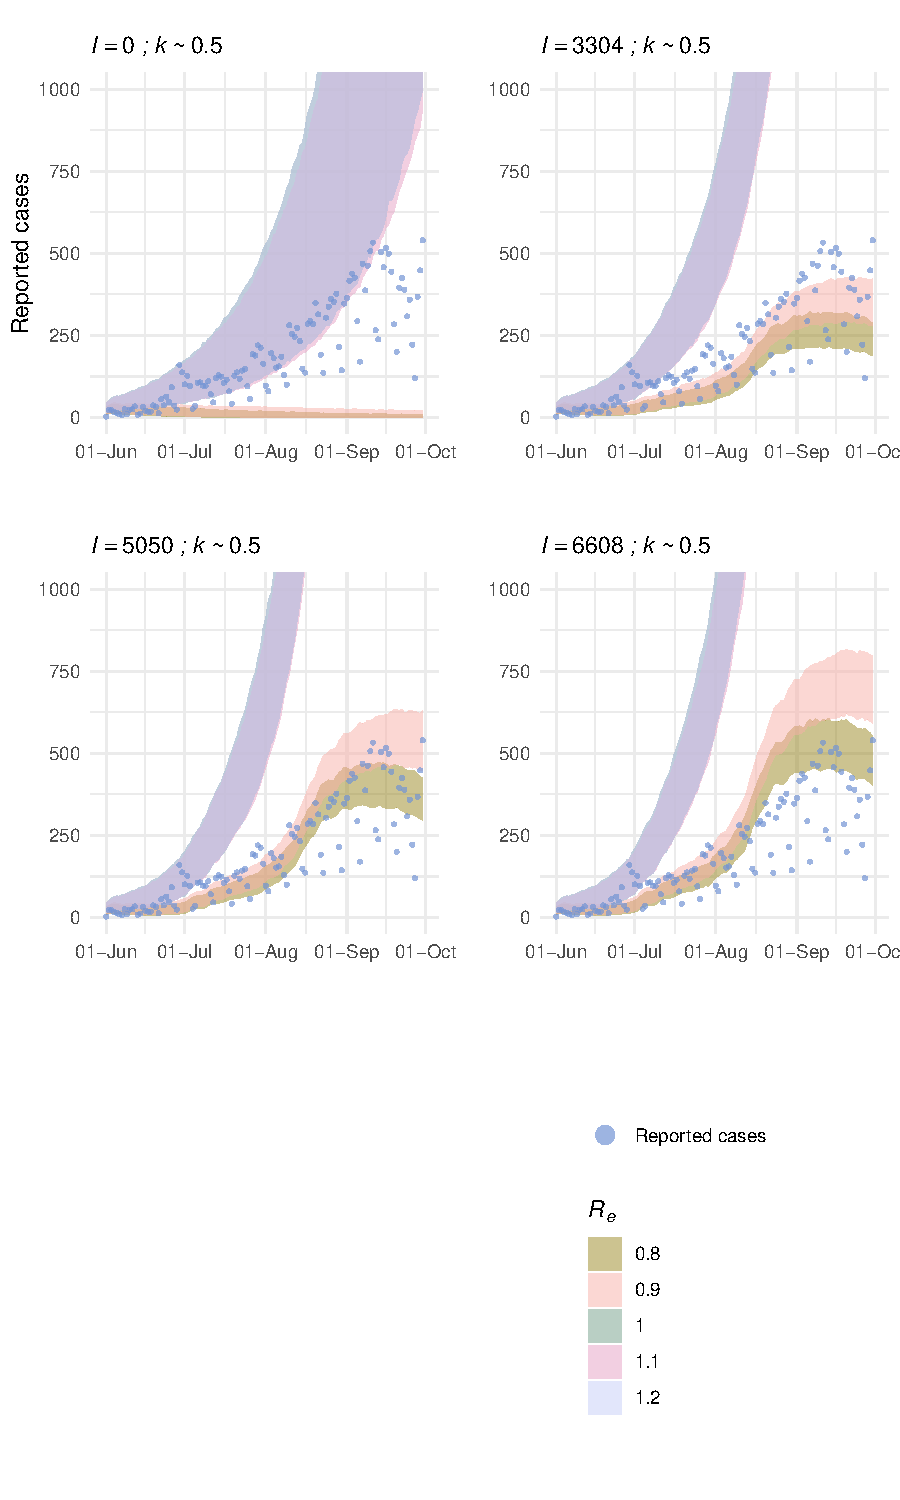
\includegraphics[scale=0.4]{SF1_2021-04-19.pdf}
\caption{Impact of cross-border-associated cases on the cases per day that infected further: y-axis cases per day; x-axis the time of interest. Different number of cross-border-associated cases \emph{I} were added to a stochastic branching model whereby these \emph{I} could transmit further: \emph{I} was zero, reported \emph{I}, reported \emph{I} multiplied by $1+ \frac{\Sigma ~of ~cases ~with ~unknown ~origin }{\Sigma ~of ~all ~confirmed ~cases}$, and these multiplied with 2 and 3, respectively. Yellow dots show the reported cases per day. Abbreviations: k, dispersion parameter; I, number of travel associated cases.}
\label{sf1}
\end{suppfigure}

\clearpage
\begin{suppfigure}[h]
\centering
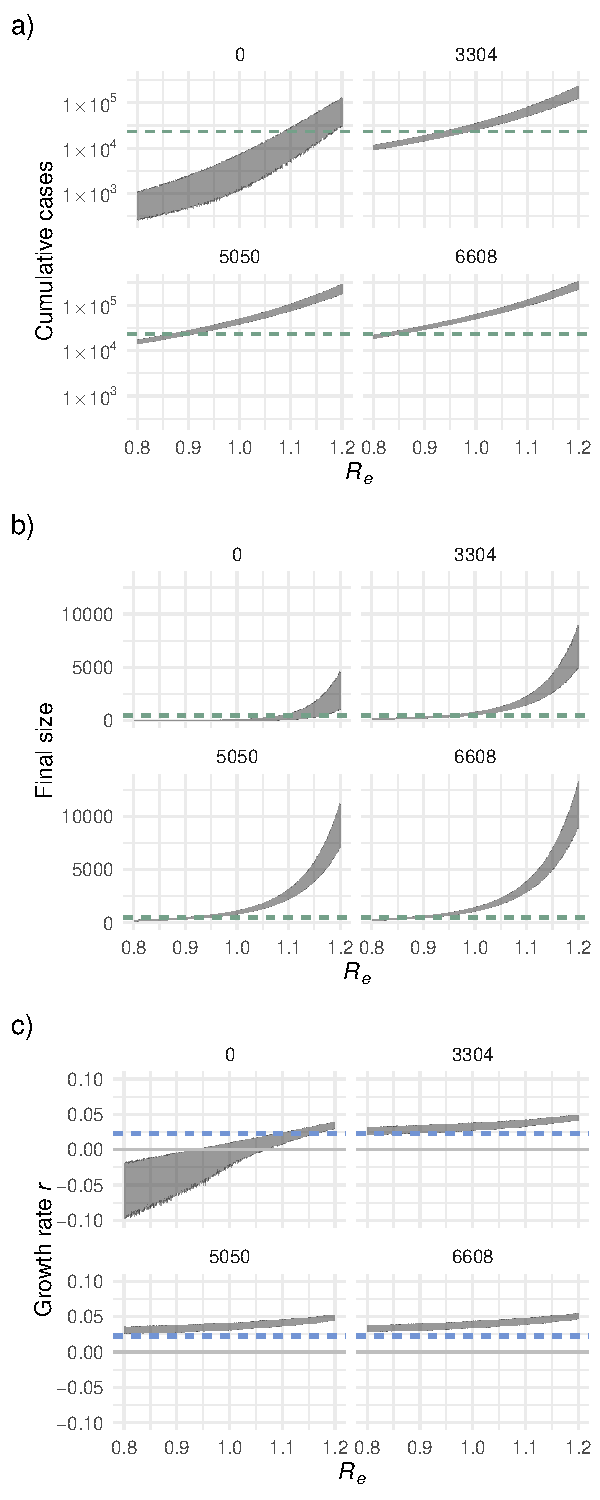
\includegraphics[scale=0.6]{SF2_2021-04-19.pdf}
\caption{a) cumulative cases b) final size c) growth rate. Dashed line shows the reported cases during $1^{st}$ of June to $30^{th}$ of September 2020 and on the $30^{th}$ of September 2020. Abbreviations: k, dispersion parameter; I, number of travel associated cases.}
\label{sf2}
\end{suppfigure}


\clearpage
\begin{suppfigure}[h]
\centering
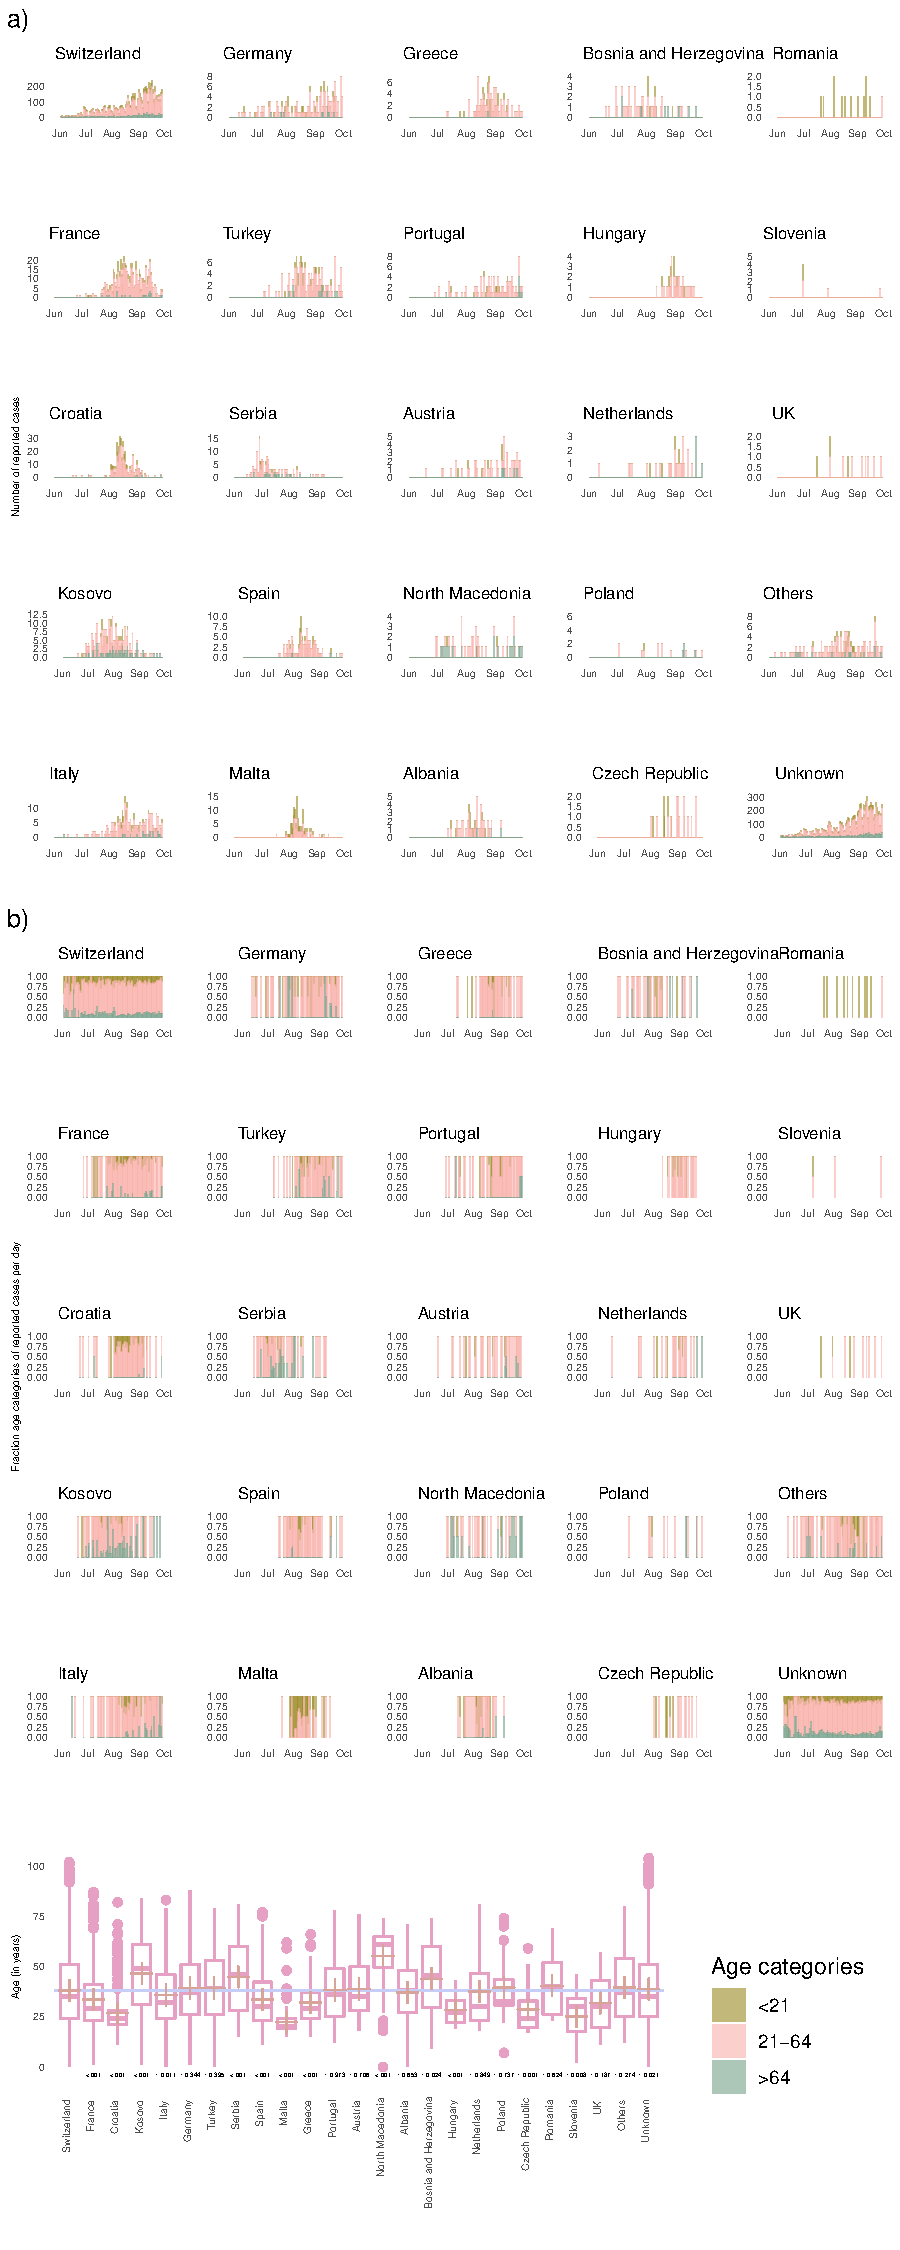
\includegraphics[scale=0.4]{SF3_2021-04-13.pdf}
\caption{Reported cases and the most likely country of exposure. a) y-axis and x-axis shows time of interest and number of reported cases and proportion of different age groups b) y-axis shows the fraction of all cases and proportion of different age groups. c) Age distribution for reported cases according to the most likely country of exposure. + represents the mean of the age in the corresponding group, the horizontal line is the mean of the age of all cases that were exposed only in Switzerland.}
\label{sf3}
\end{suppfigure}


\clearpage
\begin{suppfigure}[h]
\centering
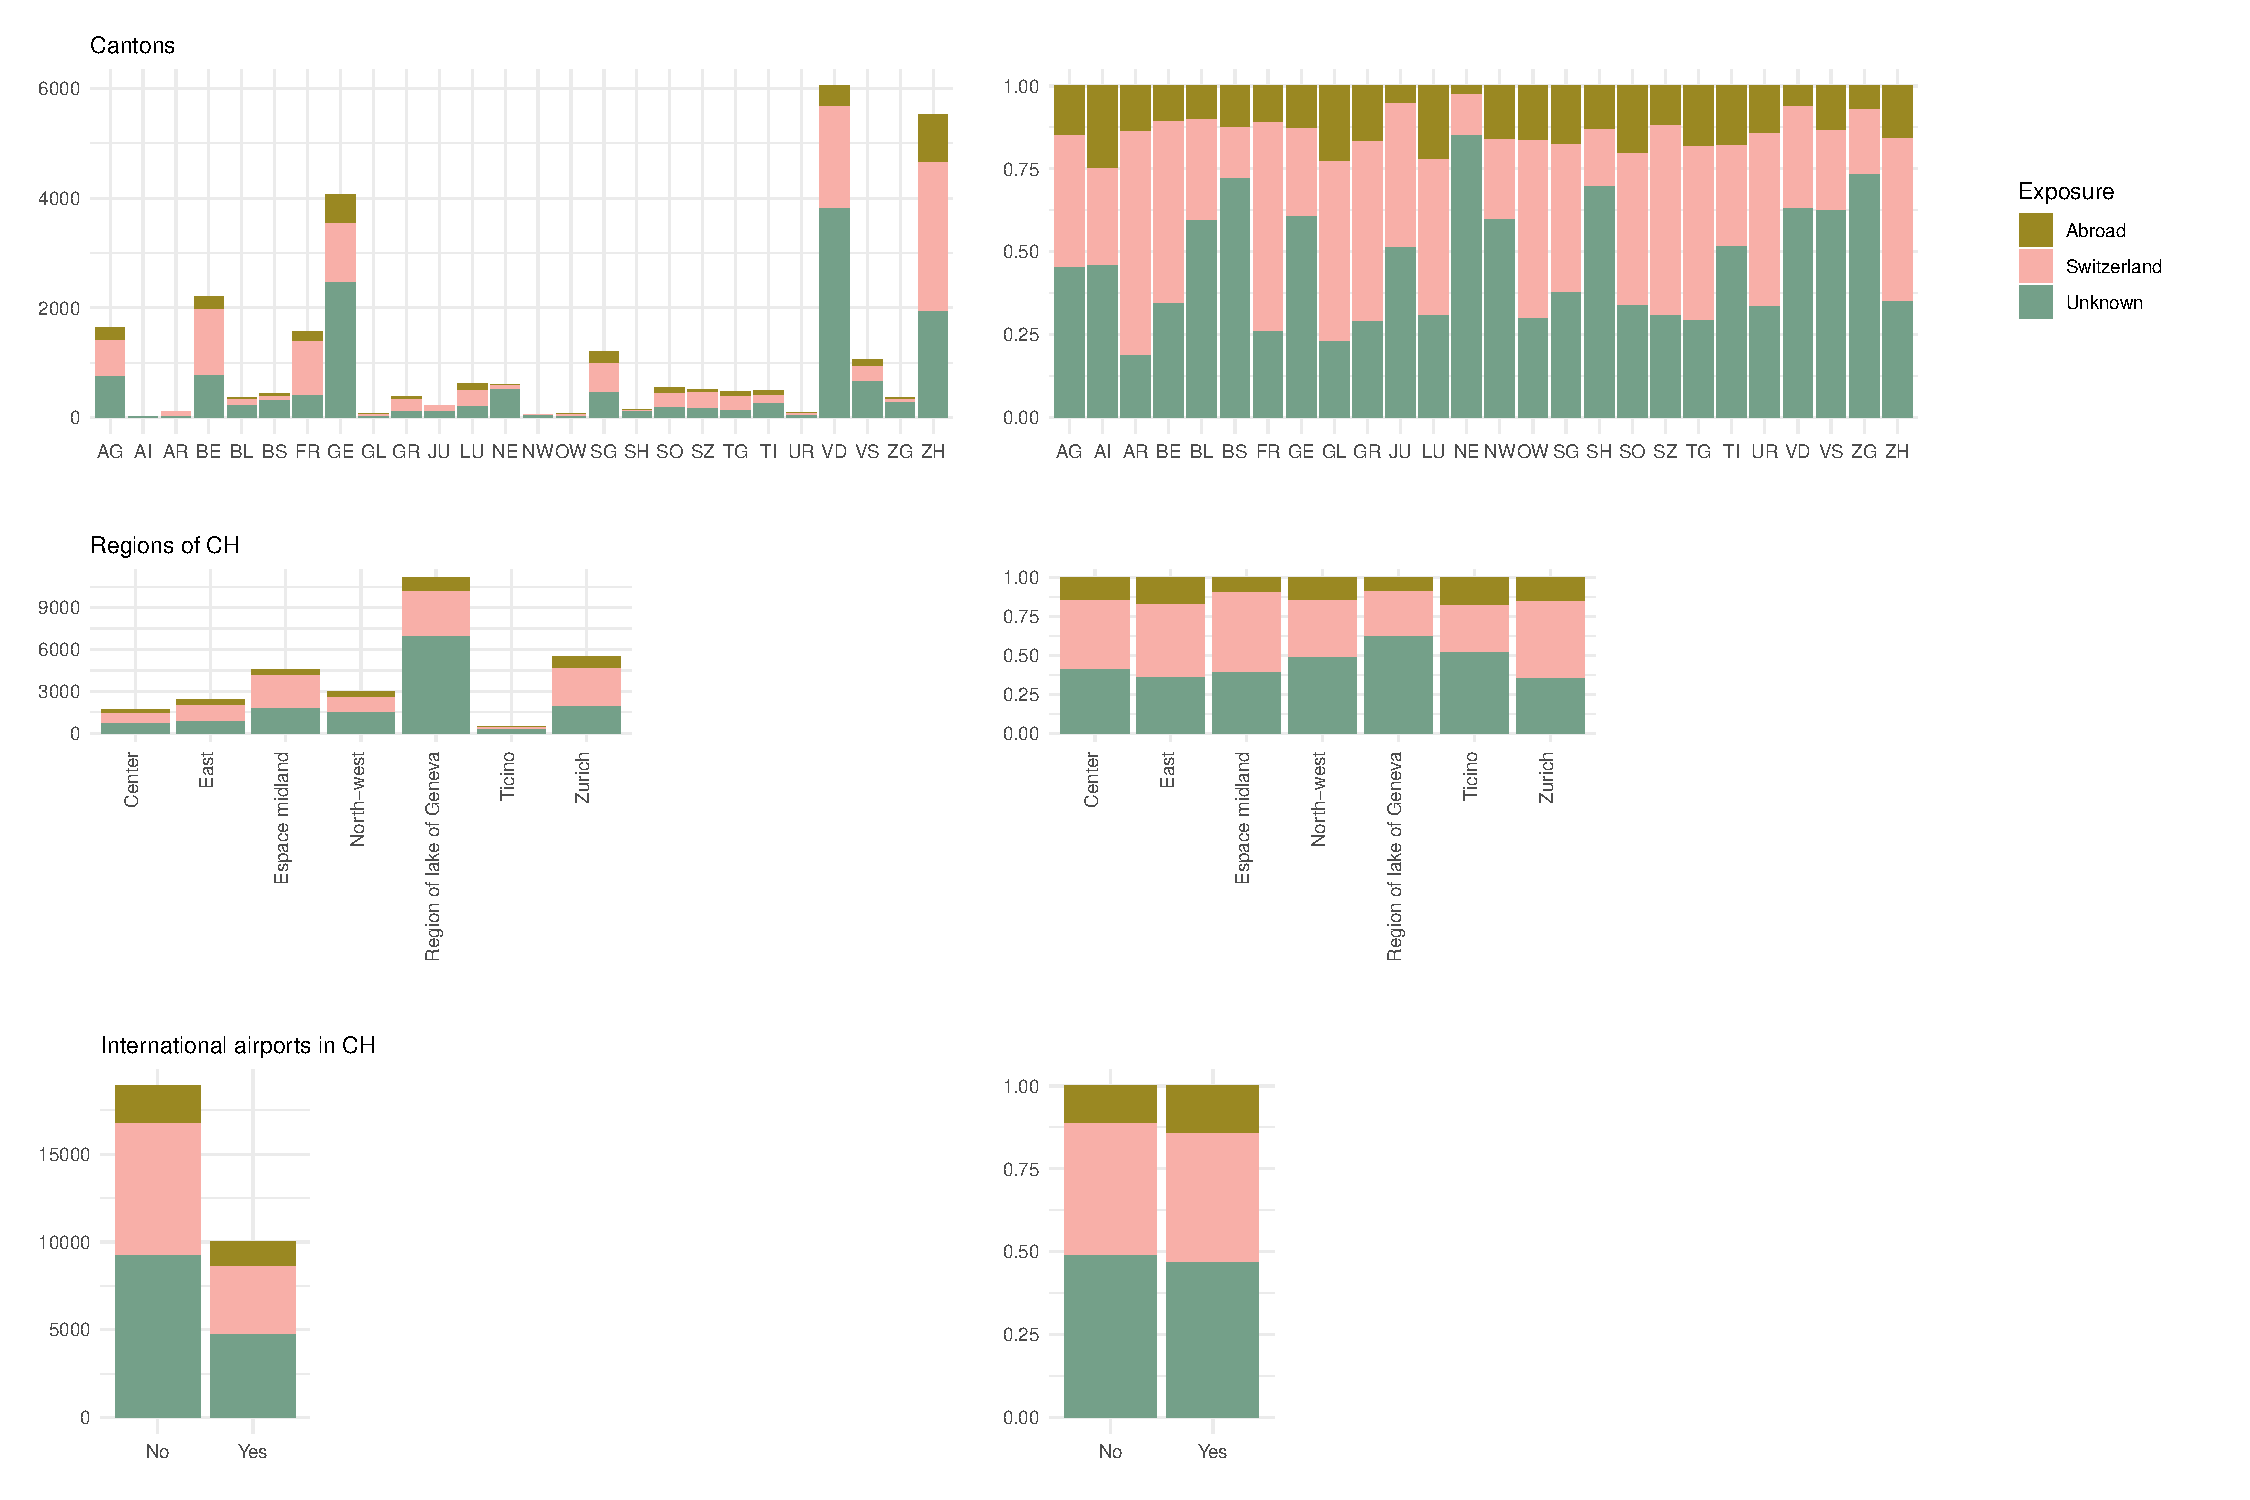
\includegraphics[scale=0.4]{SF4_2021-04-09.pdf}
\caption{Regional origin of cases that reported place of exposure}
\label{sf4}
\end{suppfigure}


\end{document}